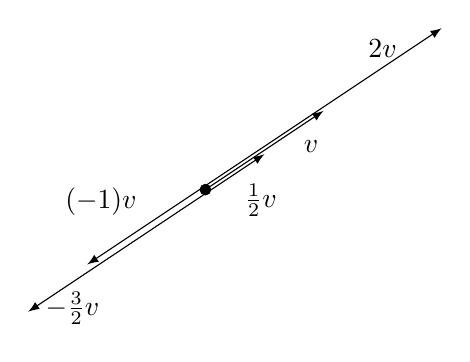
\begin{tikzpicture}[
	point/.style={circle,draw,very thin,fill,inner sep=0pt,minimum size=4pt},
	vector/.style={-latex},
]
	\node[point] at (0,0) {};
	\draw[vector] (0,0) to node[below right,near end] {$\uvec{v}$} (1.5,1);
	\draw[vector] (0,0.05) to node[above,near end] {$2\uvec{v}$} (3,2.05);
	\draw[vector] (0,0.05) to node[above left] {$(-1)\uvec{v}$} (-1.5,-0.95);
	\draw[vector] (0,-0.05) to node[below right] {$\frac{1}{2}\uvec{v}$} (0.75,0.45);
	\draw[vector] (0,-0.05) to node[below,near end] {$-\frac{3}{2}\uvec{v}$} (-2.25,-1.55);
\end{tikzpicture}
